\chapter{Model Development and Evaluation}
This section will cover the techniques used for developing models and evaluating their performance, including preprocessing methods such as scaling and transformation. It will also compare different machine learning algorithms for model development and training, including Logistic Regression, Support Vector Machines (SVM), Random Forest, and Boosting algorithms.


%%
%% Logistic Regression
%%
\section{Logistic Regression}
The data was initially split into training and testing sets, and then a log transformation was applied to the data followed by standard scaling. The resulting transformed data was used as input to a logistic regression model. During model development, different parameter and hyperparameter combinations were tested for the logistic regression model.

The hyperparameters and evaluation metrics of the model are given below:

\begin{table}[H]
    \begin{center}
        \begin{tabular}{ |c|c|c|c|c| }
            \hline
            multi\_class &
            solver       & micro avg & macro avg & weighted avg        \\
            \hline
            ovr          & newton-cg & 0.64      & 0.49         & 0.62 \\
            \hline
            multinomial  & newton-cg & 0.66      & 0.53         & 0.65 \\
            \hline
        \end{tabular}
    \end{center}
    \caption{Logistic regression hyperparameter and evaluation}
    \label{table:}
\end{table}

\begin{figure}[H]
    \centering
    \begin{subfigure}[b]{0.4\textwidth}
        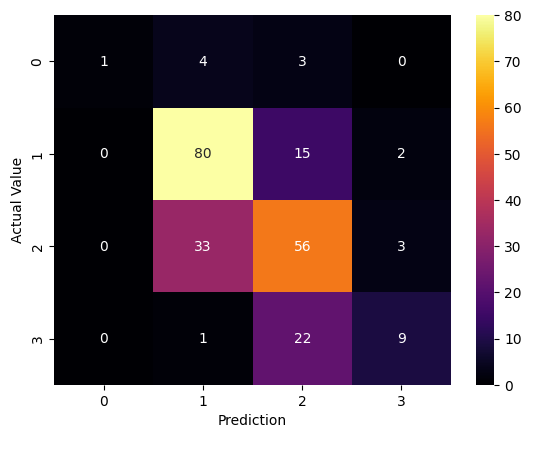
\includegraphics[width=\textwidth]{model_evaluation/logistic/cm_logistic_v3.png}
        \caption{Confusion matrix}
    \end{subfigure}
    \hfill
    \begin{subfigure}[b]{0.4\textwidth}
        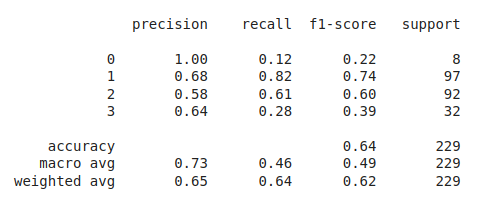
\includegraphics[width=\textwidth]{model_evaluation/logistic/cr_logistic_v3.png}
        \caption{Classification report}
    \end{subfigure}
    \caption{Confusion matrix and classification report for logistic regression model with multi\_class = "ovr"}
\end{figure}

\begin{figure}[H]
    \centering
    \begin{subfigure}[b]{0.4\textwidth}
        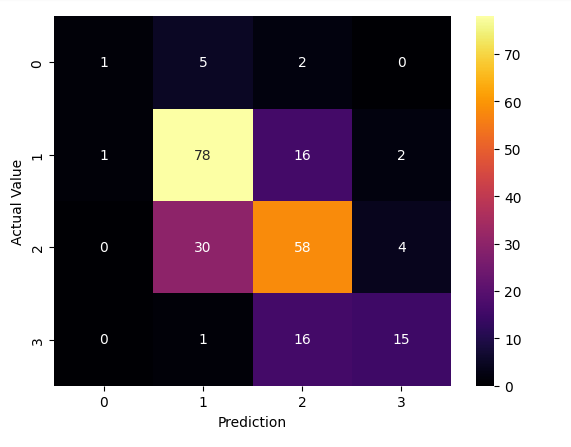
\includegraphics[width=\textwidth]{model_evaluation/logistic/cm_logistic_v2.png}
        \caption{Confusion matrix}
    \end{subfigure}
    \hfill
    \begin{subfigure}[b]{0.4\textwidth}
        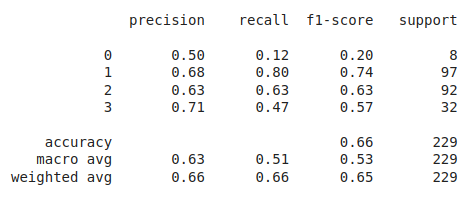
\includegraphics[width=\textwidth]{model_evaluation/logistic/cr_logistic_v2.png}
        \caption{Classification report}
    \end{subfigure}
    \caption{Confusion matrix and classification report for logistic regression model with multi\_class = "multinomial"}
\end{figure}

Smote oversampling was used to handle the imbalanced data. But the accuracy got worse instead. The results after the oversampling was as follow:


\begin{figure}[H]
    \centering
    \begin{subfigure}[b]{0.5\textwidth}
        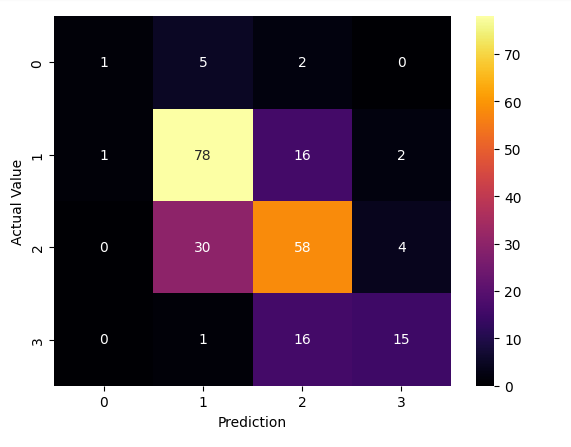
\includegraphics[width=\textwidth]{model_evaluation/logistic/cm_logistic_v2.png}
        \caption{Confusion matrix}
    \end{subfigure}
    \hfill
    \begin{subfigure}[b]{0.4\textwidth}
        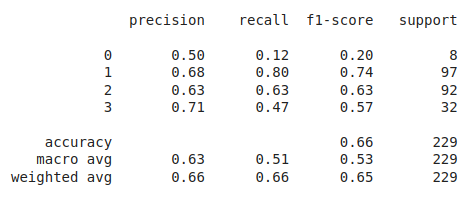
\includegraphics[width=\textwidth]{model_evaluation/logistic/cr_logistic_v2.png}
        \caption{Classification report}
    \end{subfigure}
    \caption{Confusion matrix and classification report for logistic regression model after smote oversampling}
\end{figure}


%%
%% Boosting
%%
\section{Boosting}
To develop models using boosting algorithms, the initial step was to split the data into training and testing sets. After that, the training dataset was oversampled using the SMOTE technique.

The next step involved fitting a min-max scaler to the training data, and then scaling both the training and testing data using this scaler. A log transformation was then applied to the preprocessed data.

Various boosting algorithms such as XGBClassifier and AdaBoost were utilized to train models on the preprocessed training data. The performance of these models was then assessed, and the best performing algorithm was determined.

\subsection{XGBClassifier}
The RandomizedSearchCV was used to tune the hyperparameters of the XGBClassifier. The results were as follow:

\begin{table}[H]
    \begin{center}
        \begin{tabular}{ |c|c|c|c|c|c|c|c| }
            \hline
            id      & learning\_rate & max\_depth & n\_estimators & subsample & micro & macro & weighted \\
            \hline
            xgb\_v1 & 0.0824         & 16         & 113           & 0.5394    & 0.64  & 0.49  & 0.65     \\
            \hline
            xgb\_v2 & 0.0903         & 19         & 127           & 0.6520    & 0.63  & 0.48  & 0.63     \\
            \hline
        \end{tabular}
    \end{center}
    \caption{XGBClassifier hyperparameter and evaluation metrics}
\end{table}

\begin{figure}[H]
    \centering
    \begin{subfigure}[b]{0.5\textwidth}
        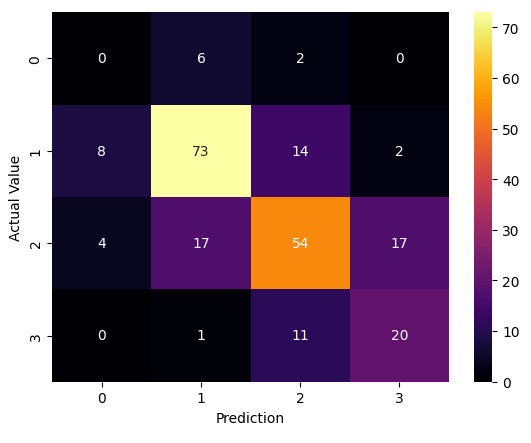
\includegraphics[width=\textwidth]{model_evaluation/boosting/cm_xgb_v1.png}
        \caption{Confusion matrix}
    \end{subfigure}
    \hfill
    \begin{subfigure}[b]{0.4\textwidth}
        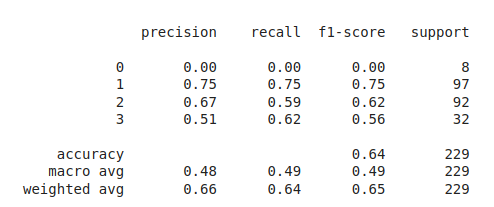
\includegraphics[width=\textwidth]{model_evaluation/boosting/cr_xgb_v1.png}
        \caption{Classification report}
    \end{subfigure}
    \caption{Confusion matrix and classification report for XGBClassifier xgb\_v1}
\end{figure}

\begin{figure}[H]
    \centering
    \begin{subfigure}[b]{0.5\textwidth}
        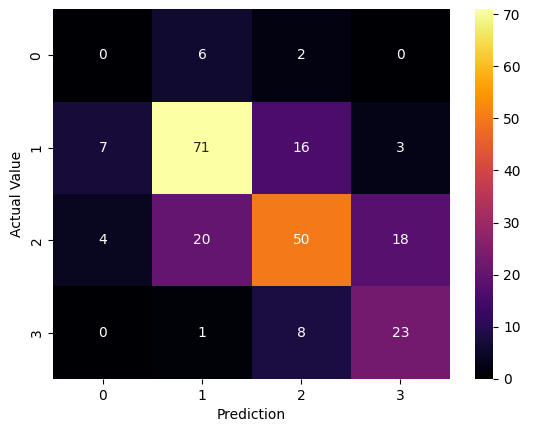
\includegraphics[width=\textwidth]{model_evaluation/boosting/cm_xgb_v2.png}
        \caption{Confusion matrix}
    \end{subfigure}
    \hfill
    \begin{subfigure}[b]{0.4\textwidth}
        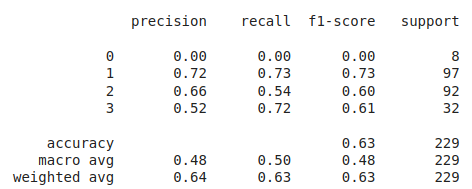
\includegraphics[width=\textwidth]{model_evaluation/boosting/cr_xgb_v2.png}
        \caption{Classification report}
    \end{subfigure}
    \caption{Confusion matrix and classification report for XGBClassifier xgb\_v2}
\end{figure}

\subsection{AdaBoost, Gradient Boosting and LGBMClassifier}
The same preprocessing step were followed and the results were as follow:


\begin{table}[H]
    \begin{center}
        \begin{tabular}{ |c|c|c|c| }
            \hline
            model   & micro & macro & weighted \\
            \hline
            AdaBoost & 0.51  & 0.46  & 0.55     \\
            \hline
            Gradient Boosting & 0.61  & 0.50  & 0.61     \\
            \hline
            xgb\_v1 & 0.64  & 0.49  & 0.65     \\
            \hline
        \end{tabular}
    \end{center}
    \caption{Boosting algorithms evaluation metrics}
\end{table}

\begin{figure}[H]
    \centering
    \begin{subfigure}[b]{0.5\textwidth}
        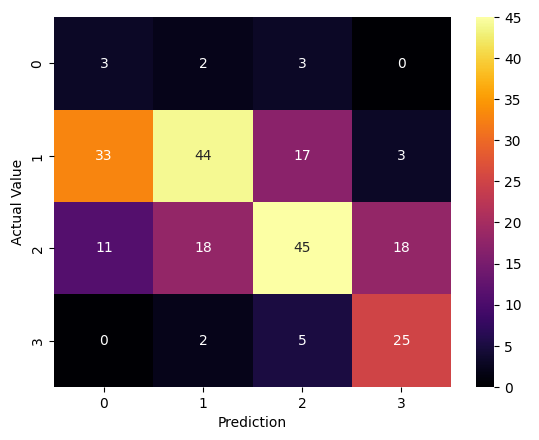
\includegraphics[width=\textwidth]{model_evaluation/boosting/cm_ada.png}
        \caption{Confusion matrix}
    \end{subfigure}
    \hfill
    \begin{subfigure}[b]{0.4\textwidth}
        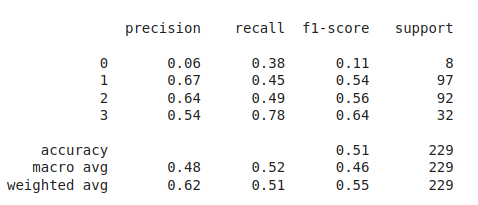
\includegraphics[width=\textwidth]{model_evaluation/boosting/cr_ada.png}
        \caption{Classification report}
    \end{subfigure}
    \caption{Confusion matrix and classification report for AdaBoost}
\end{figure}

\begin{figure}[H]
    \centering
    \begin{subfigure}[b]{0.5\textwidth}
        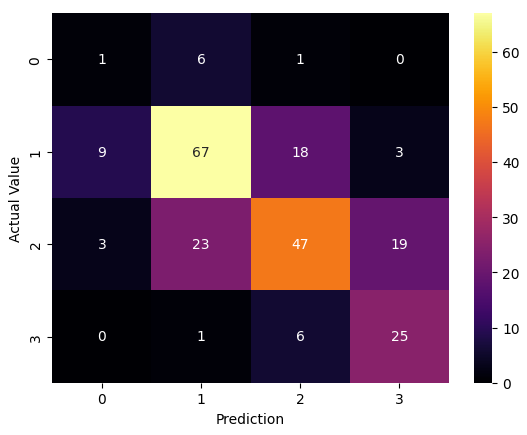
\includegraphics[width=\textwidth]{model_evaluation/boosting/cm_gradient.png}
        \caption{Confusion matrix}
    \end{subfigure}
    \hfill
    \begin{subfigure}[b]{0.4\textwidth}
        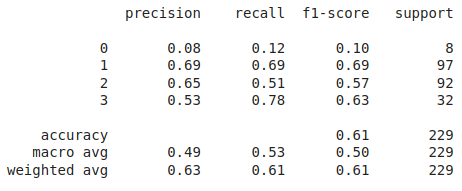
\includegraphics[width=\textwidth]{model_evaluation/boosting/cr_gradient.png}
        \caption{Classification report}
    \end{subfigure}
    \caption{Confusion matrix and classification report for Gradient Boosting Classifier}
\end{figure}

\begin{figure}[H]
    \centering
    \begin{subfigure}[b]{0.5\textwidth}
        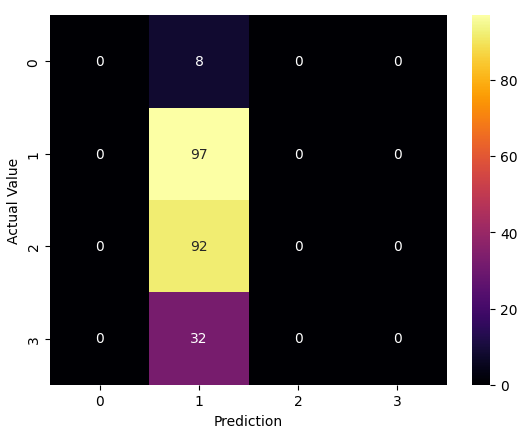
\includegraphics[width=\textwidth]{model_evaluation/boosting/cm_lgbm.png}
        \caption{Confusion matrix}
    \end{subfigure}
    \hfill
    \begin{subfigure}[b]{0.4\textwidth}
        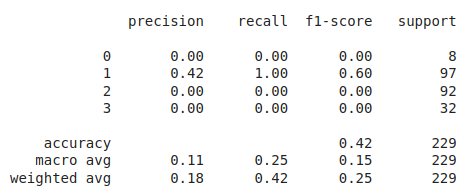
\includegraphics[width=\textwidth]{model_evaluation/boosting/cr_lgbm.png}
        \caption{Classification report}
    \end{subfigure}
    \caption{Confusion matrix and classification report for LGBM Classifier}
\end{figure}

\section{Random Forest and SVM}
The first step in developing models using random forest and SVM classifiers involved splitting the data into training and testing sets. Next, a log transformation was applied to the data to normalize it.

After normalization, the data was scaled using the Robust Scaler, which was specifically chosen for its ability to handle outliers in the data. The preprocessed data was then used to train models using the random forest and SVM classifiers.


%%
%% Random Forest
%%
\subsection{Random Forest}
The hyperparameter tuning result and evaluation metrics for each model are shown below.

\begin{table}[H]
    \begin{center}
        \begin{tabular}{ |c|c|c|c|c|c|c|c| }
            \hline
            id & n\_estimators & max\_depth & min\_samples\_split & min\_samples\_leaf  & micro & macro & weighted \\
            \hline
            1 & 100 & None  & None  & 1 & 0.73  & 0.54  & 0.72     \\
            \hline        
            2 & 200 & 20  & 2  & 1 & 0.69  & 0.51  & 0.68     \\
            \hline
        \end{tabular}
    \end{center}
    \caption{Random Forest hyperparameters and evaluation metrics}
\end{table}

\begin{figure}[H]
    \centering
    \begin{subfigure}[b]{0.5\textwidth}
        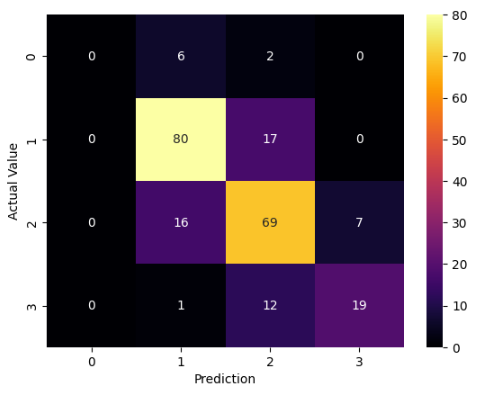
\includegraphics[width=\textwidth]{model_evaluation/rf_svm/cm_rf_v1.png}
        \caption{Confusion matrix}
    \end{subfigure}
    \hfill
    \begin{subfigure}[b]{0.4\textwidth}
        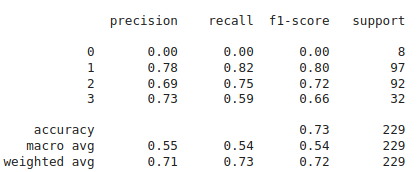
\includegraphics[width=\textwidth]{model_evaluation/rf_svm/cr_rf_v1.png}
        \caption{Classification report}
    \end{subfigure}
    \caption{Confusion matrix and classification report for Random Forest Classifier 1}
\end{figure}

\begin{figure}[H]
    \centering
    \begin{subfigure}[b]{0.5\textwidth}
        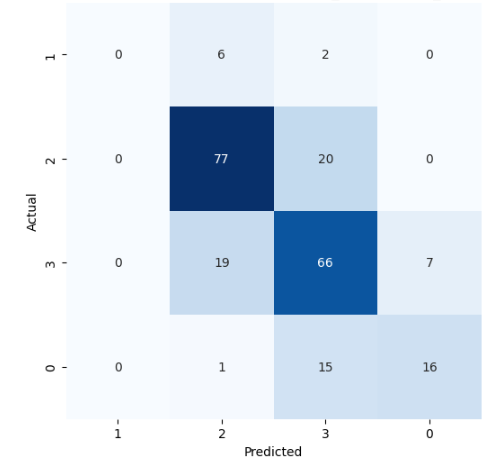
\includegraphics[width=\textwidth]{model_evaluation/rf_svm/cm_rf_v2.png}
        \caption{Confusion matrix}
    \end{subfigure}
    \hfill
    \begin{subfigure}[b]{0.4\textwidth}
        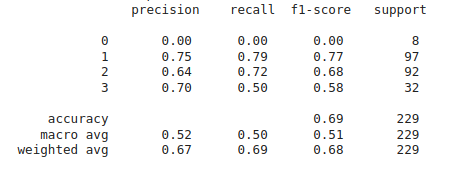
\includegraphics[width=\textwidth]{model_evaluation/rf_svm/cr_rf_v2.png}
        \caption{Classification report}
    \end{subfigure}
    \caption{Confusion matrix and classification report for Random Forest Classifier 2}
\end{figure}


%%
%% SVM
%%
\section{SVM}
The hyperparameter tuning result and evaluation metrics for each model are shown below.
\begin{table}[H]
    \begin{center}
        \begin{tabular}{ |c|c|c|c|c|c|c|c| }
            \hline
            id & C & kernel &  micro & macro & weighted \\
            \hline
            1 & 1 & ovr & 0.67 & 0.46  & 0.65     \\
            \hline        
            2 & 1 & linear  & 0.62  & 0.44 & 0.61     \\
            \hline
        \end{tabular}
    \end{center}
    \caption{SVM hyperparameters and evaluation metrics}
\end{table}


\begin{figure}[H]
    \centering
    \begin{subfigure}[b]{0.5\textwidth}
        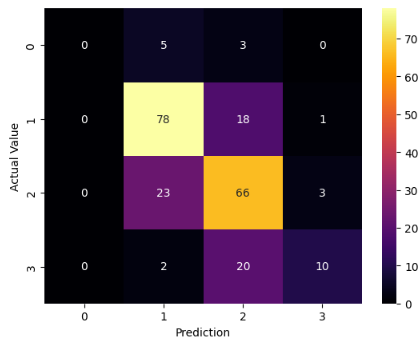
\includegraphics[width=\textwidth]{model_evaluation/rf_svm/cm_svm_v1.png}
        \caption{Confusion matrix}
    \end{subfigure}
    \hfill
    \begin{subfigure}[b]{0.4\textwidth}
        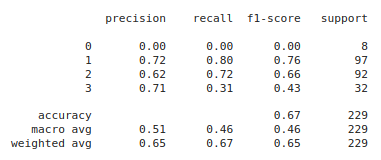
\includegraphics[width=\textwidth]{model_evaluation/rf_svm/cr_svm_v1.png}
        \caption{Classification report}
    \end{subfigure}
    \caption{Confusion matrix and classification report for SVM id = 1}
\end{figure}


\begin{figure}[H]
    \centering
    \begin{subfigure}[b]{0.5\textwidth}
        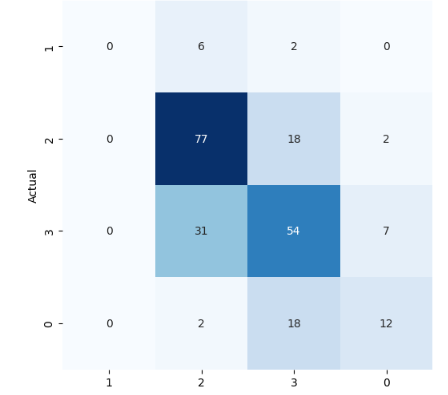
\includegraphics[width=\textwidth]{model_evaluation/rf_svm/cm_svm_v2.png}
        \caption{Confusion matrix}
    \end{subfigure}
    \hfill
    \begin{subfigure}[b]{0.4\textwidth}
        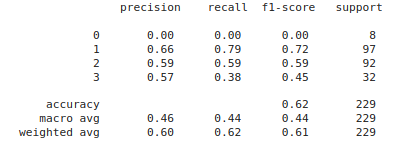
\includegraphics[width=\textwidth]{model_evaluation/rf_svm/cr_svm_v2.png}
        \caption{Classification report}
    \end{subfigure}
    \caption{Confusion matrix and classification report for SVM id = 2}
\end{figure}







